\documentclass{article}
% \usepackage{xeCJK}
\usepackage{amsmath}
\usepackage{amssymb}
\usepackage{mathrsfs}
\usepackage{xcolor}
\usepackage{bm}
\usepackage{hyperref}
\usepackage{graphicx}
\usepackage{subcaption}
\usepackage{float}
\usepackage{multicol}
\usepackage[ruled,linesnumbered]{algorithm2e}

\bibliographystyle{plain}
\setlength{\parindent}{2em}
\usepackage{geometry}
\geometry{a4paper, left=2.54cm, right=2.54cm, top=3.18cm, bottom=3.18cm}

% 设置文章行距
% \renewcommand{\baselinestretch}{1.5}

% define reference format
\hypersetup{
    colorlinks=true,
    linkcolor=blue,
    urlcolor=blue,
    citecolor=blue,
    linkbordercolor=white
}

\title{\textbf{Chemotactic Chiral Active Matter}}
\author{Yichen Lu}

\begin{document}

\maketitle

\tableofcontents

\newpage
\section{Models}
\subsection{Definitions}
\subsubsection{General Model}
\begin{subequations}
    \begin{align}
        &\dot{\mathbf{r}}_i\left( t \right) =v\mathbf{p}\left( \theta _i \right) +\sum_{j\in A_{i}^{1,2}}{\mathbf{I}\left( \Delta \mathbf{r}_{ij} \right)}\;,\\
        &\dot{\theta}_i\left( t \right) =\omega _i+G\left( \mathbf{r},\theta ,c \right) +\sum_{j\ne i}{H\left( \Delta \theta _{ij},\Delta \mathbf{r}_{ij} \right)}\;,\\
        &\dot{c}\left( \mathbf{r},t \right) =D\nabla ^2c+F\left( c \right) \sum_{j=1}{\delta \left( \mathbf{r}-\mathbf{r}_i \right)}\;,
    \end{align}
\end{subequations}
for $i=1,2,\cdots,N$. Here, $\mathbf{r}_i$ is the position of the $i$-th particle, $\theta _i$ is the orientation of the $i$-th particle, $v$ is the self-propulsion velocity, $\mathbf{p}\left( \theta _i \right)=\left( \cos \theta _i,\sin \theta _i \right)$ is the unit vector pointing in the direction of the $i$-th particle, $\omega _i$ is the natural frequency of the $i$-th particle, $G\left( \mathbf{r},\theta ,c \right)$ is the coupling function between particles and chemical fields, $H\left( \Delta \theta _{ij},\Delta \mathbf{r}_{ij} \right)$ is the coupling function between partials, $c\left( \mathbf{r},t \right)$ is the chemical concentration, $D$ is the diffusion coefficient, $F\left( c \right)$ is the production rate of the chemical field, $A_{i}^{1,2}=\left\{ j\mid r_c\geqslant | \mathbf{r}_j-\mathbf{r}_i | \right\}$, $\Delta \mathbf{r}_{ij}=\mathbf{r}_j-\mathbf{r}_i$, $\Delta \theta _{ij}=\theta _j-\theta _i$, $\mathbf{I}\left( \Delta \mathbf{r}_{ij} \right)=\frac{\Delta \mathbf{r}_{ij}}{|\Delta \mathbf{r}_{ij}|^{2}}$.
The natural frequencies $\omega_i$ are distributed with following two cases:
\begin{enumerate}
    \item \textbf{Single-chiral particles:} The natural frequencies $\omega_i$ are distributed in $U\left( \omega _{\min},\omega _{\max} \right)$ for all particles and $\omega _{\min}\omega _{\max}>0$.
    
    \item \textbf{Double-chiral particles:} The frequencies are distributed in two symmetric uniform distributions, representing two types of chirality. Exactly half of the particles have natural frequencies $\omega_i \sim U\left( \omega _{\min},\omega _{\max} \right)$ and the other half have natural frequencies $\omega_i \sim U\left( -\omega _{\max},-\omega _{\min} \right)$.
\end{enumerate}

\subsubsection{Polar alignment Interaction}
\begin{itemize}
    \item Additive coupling: 
    \begin{equation}
        \label{eq:additionalCouplingDotTheta}
        \dot{\theta}_i=\omega _i+K\sum_{j=1}^{N}f\left( r_{ij} \right)\sin \left( \theta _j-\theta _i+\alpha \right)\;,
    \end{equation}
    \item Mean-field coupling by oscillator number:
    \begin{equation}
        \label{eq:particleDotTheta}
        \dot{\theta}_i=\omega _i+\frac{K}{N}\sum_{j=1}^N{f}\left( r_{ij} \right) \sin \left( \theta _j-\theta _i+\alpha \right) \;,
    \end{equation}
\end{itemize}
Here,  $f\left( r_{ij} \right)$ is a function of $r=\left| \mathbf{r}_i-\mathbf{r}_j \right|$, and $K$ is the coupling strength. 
The function $f\left( r \right)$ can be defined as
\begin{enumerate}
    \item $f_H\left( r \right)=H\left( d_0-r \right),\;r_0>0$;
    \item $f_E\left( r \right)=e^{-\frac{r}{d_0}},\;r_0>0$.
\end{enumerate}

\subsubsection{Chemotactic Interaction}
\noindent\textbf{General Chemotactic Model For Two Species}

\noindent\textcolor{red}{Type 1:}
\begin{subequations}
    \begin{align}
        &\dot{\mathbf{r}}_{i}^{1,2}=v\mathbf{p}\left( \theta _{i}^{1,2} \right) -\sum_{j\in A_{i}^{1,2}}{\mathbf{I}_{ij}^{1,2}\;,}\\
        &\dot{\theta}_{i}^{1,2}=\omega + \left| \nabla c_{1,2} \right|\sin \left( \varphi _{c_{1,2}}-\theta _{i}^{1,2} \right) +F\left( \theta ,\mathbf{r} \right) \;,\\
        &\dot{c}_1=D_1\nabla ^2c_1+F_1\left( c_1,c_2 \right) \sum_{j=1}^N{\delta \left( \mathbf{r}-\mathbf{r}_{j}^{1} \right) \;,}\\
        &\dot{c}_2=D_2\nabla ^2c_2+F_2\left( c_1,c_2 \right) \sum_{j=1}^N{\delta \left( \mathbf{r}-\mathbf{r}_{j}^{2} \right) \;,}
    \end{align}
\end{subequations}
where $\mathbf{I}_{ij}^{1,2}=\frac{\mathbf{r}_j-\mathbf{r}_{i}^{1,2}}{|\mathbf{r}_j-\mathbf{r}_{i}^{1,2}|^{2}}$, $\varphi _{c_{1,2}}=\arctan \left( \frac{\partial _yc_{1,2}}{\partial _xc_{1,2}} \right) $ and $A_{i}^{1,2}=\left\{ j\mid r_c\geqslant | \mathbf{r}_j-\mathbf{r}_{i}^{1,2} | \right\}$.

\noindent Type 2:
\begin{subequations}
    \begin{align}
        &\dot{\mathbf{r}}_{i}^{1,2}=v\mathbf{p}\left( \theta _{i}^{1,2} \right) +\alpha _{1,2}\nabla c_{1,2}-\sum_{j\in A_{i}^{1,2}}{\mathbf{I}_{ij}^{1,2}\;,}\\
        &\dot{\theta}_{i}^{1,2}=\omega + F\left( \theta ,\mathbf{r} \right) \;,\\
        &\dot{c}_1=D_1\nabla ^2c_1+F_1\left( c_1,c_2 \right) \sum_{j=1}^N{\delta \left( \mathbf{r}-\mathbf{r}_{j}^{1} \right) \;,}\\
        &\dot{c}_2=D_2\nabla ^2c_2+F_2\left( c_1,c_2 \right) \sum_{j=1}^N{\delta \left( \mathbf{r}-\mathbf{r}_{j}^{2} \right) \;,}
    \end{align}
\end{subequations}

\noindent\textbf{Chemotactic Model with Lotka-Volterra Functions}

Let $F_1\left( c_1,c_2 \right)=c_1\left( k_1-k_2c_2 \right)$ and $F_2\left( c_1,c_2 \right)=c_2\left( k_3c_1-k_4 \right)$, where $k_1,k_2,k_3,k_4$ are constants.

\begin{subequations}
    \begin{align}
        &\dot{\mathbf{r}}_{i}^{1,2}=v\mathbf{p}\left( \theta _{i}^{1,2} \right) -\sum_{j\in A_{i}^{1,2}}{\mathbf{I}_{ij}^{1,2}\;,}\label{dotR}\\
        &\dot{\theta}_{i}^{1,2}=\omega + \left| \nabla c_{1,2} \right|\sin \left( \varphi _{c_{1,2}}-\theta _{i}^{1,2} \right) +F\left( \theta ,\mathbf{r} \right) \;,\label{dotTheta}\\
        &\dot{c}_1=D_1\nabla ^2c_1+c_1\left( k_1-k_2c_2 \right) \sum_{j=1}^N{\delta \left( \mathbf{r}-\mathbf{r}_{j}^{1} \right) \;,}\\
        &\dot{c}_2=D_2\nabla ^2c_2+c_2\left( k_3c_1-k_4 \right) \sum_{j=1}^N{\delta \left( \mathbf{r}-\mathbf{r}_{j}^{2} \right) \;,}
    \end{align}
    \label{eq:chemoLVModel}
\end{subequations}

\section{Continuum model}
We start with the model as given by Eqs. \eqref{eq:chemoLVModel} in the main text but replace the finite range alignment interaction by a pseudopotential ($\delta$-interaction), which is justified if the interaction is short ranged enough, such that the shape of the associated interaction potential is irrelevant to the many particle dynamics:

In the thermodynamic limit $N\rightarrow \infty$, the Eqs.~\eqref{dotR} and \eqref{dotTheta} give rise to the following continuum model:
\begin{equation}
    \frac{\partial}{\partial t}f ^{1,2}\left( \mathbf{r},\theta ,t \right) =-\frac{\partial}{\partial \theta}\left( f ^{1,2}v_{\theta}^{1,2} \right) -\nabla \cdot \left( f ^{1,2}\mathbf{v}_{\mathbf{r}}^{1,2} \right) \;, \label{eq:continuumModel}
\end{equation}
where $f^{1,2}\left( \mathbf{r},\theta ,t \right)$ is the probability density of particles of species 1 or 2 at position $\mathbf{r}$ and orientation $\theta$ at time $t$, and $\mathbf{v}_{\mathbf{r}}^{1,2}$ and $v_{\theta}^{1,2}$ are the velocity fields in the position and orientation space, respectively. The velocity fields are given by
\begin{subequations}
    \begin{align}
        &v_{\theta}^{1,2}\left( \mathbf{r},\theta ,t \right) =\omega +\left| \nabla c_{1,2} \right|\sin \left( \varphi _{c_{1,2}} -\theta \right) +F\left( \theta ,\mathbf{r} \right)  \;,\\
        &\mathbf{v}_{\mathbf{r}}^{1,2}\left( \mathbf{r},\theta ,t \right) =v\mathbf{p}\left( \theta \right) -\int{\mathrm{d}\theta ^{\prime} \mathrm{d}\mathbf{r}^{\prime} f ^{1,2}\left( \mathbf{r}^{\prime} ,\theta ^{\prime} ,t \right) \mathbf{I}\left( \mathbf{r}^{\prime}-\mathbf{r} \right)} \;,
    \end{align}
    \label{eq:velocityFields}
\end{subequations}
where $\mathbf{I}\left( \mathbf{r} \right)=|\mathbf{r}|^{-2}\mathbf{r}$. By substituting Eqs.~\eqref{eq:velocityFields} into Eq.~\eqref{eq:continuumModel}, we obtain
\begin{equation}
    \begin{aligned}
        \frac{\partial}{\partial t}f ^{1,2}\left( \mathbf{r},\theta ,t \right) =&-v\mathbf{p}\left( \theta \right) \cdot \nabla f ^{1,2}-\nabla \cdot \mathbf{F}^{1,2}\left( \mathbf{r},\theta ,t \right) \\
        &-\omega \partial _{\theta}f ^{1,2}-\left| \nabla c_{1,2} \right|\partial _{\theta}\left[ f ^{1,2}\sin \left( \varphi _{c_{1,2}}-\theta \right) \right]\;,
    \end{aligned}
\end{equation}
where
\begin{equation}
    \mathbf{F}^{1,2}\left( \mathbf{r},\theta ,t \right)=\nabla \cdot \int{\mathrm{d}\theta ^{\prime}\mathrm{d}\mathbf{r}^{\prime}f^{1,2}\left( \mathbf{r}^{\prime},\theta ^{\prime},t \right) f^{1,2}\left( \mathbf{r},\theta ,t \right) \frac{\mathbf{r}^{\prime}-\mathbf{r}}{\left| \mathbf{r}^{\prime}-\mathbf{r} \right|^2}}\;,
\end{equation}
and 
\begin{equation}
    \begin{aligned}
        \nabla\cdot\mathbf{F}^{1,2}\left( \mathbf{r},\theta ,t \right) &=\nabla \cdot \int{\mathrm{d}\theta ^{\prime}\mathrm{d}\mathbf{r}^{\prime}f^{1,2}\left( \mathbf{r}^{\prime},\theta ^{\prime},t \right) f^{1,2}\left( \mathbf{r},\theta ,t \right) \frac{\mathbf{r}^{\prime}-\mathbf{r}}{\left| \mathbf{r}^{\prime}-\mathbf{r} \right|^2}}\\
        &=\int{\mathrm{d}\theta ^{\prime}\mathrm{d}\mathbf{r}^{\prime}f^{1,2}\left( \mathbf{r}^{\prime},\theta ^{\prime},t \right) \nabla \cdot \left[ f^{1,2}\left( \mathbf{r},\theta ,t \right) \frac{\mathbf{r}^{\prime}-\mathbf{r}}{\left| \mathbf{r}^{\prime}-\mathbf{r} \right|^2} \right]}\\
        &=\int{\mathrm{d}\theta ^{\prime}\mathrm{d}\mathbf{r}^{\prime}f^{1,2}\left( \mathbf{r}^{\prime},\theta ^{\prime},t \right) \left[ -2\pi \delta \left( \mathbf{r}^{\prime}-\mathbf{r} \right) f^{1,2}\left( \mathbf{r},\theta ,t \right) +\nabla f^{1,2}\left( \mathbf{r},\theta ,t \right) \cdot \frac{\mathbf{r}^{\prime}-\mathbf{r}}{\left| \mathbf{r}^{\prime}-\mathbf{r} \right|^2} \right]}\\
        &=-2\pi \left[ f^{1,2}\left( \mathbf{r},\theta ,t \right) \right] ^2+\int{\mathrm{d}\theta ^{\prime}\mathrm{d}\mathbf{r}^{\prime}f^{1,2}\left( \mathbf{r}^{\prime},\theta ^{\prime},t \right) \nabla f^{1,2}\left( \mathbf{r},\theta ,t \right) \cdot \frac{\mathbf{r}^{\prime}-\mathbf{r}}{\left| \mathbf{r}^{\prime}-\mathbf{r} \right|^2}}\\
    \end{aligned}
\end{equation}
The equation accounts for self-propulsion, and short-range repulsion between particles, rotational diffusion and chemotactic alignment.
From here, we expand $f^{1,2}\left( \mathbf{r},\theta ,t \right)$ in a Fourier series 
\begin{equation}
    f ^{1,2}\left( \mathbf{r},\theta ,t \right) =\sum_{k=-\infty}^{\infty}{f _{k}^{1,2}\left( \mathbf{r},t \right) \mathrm{e}^{\mathrm{i}k\theta}}\;,
\end{equation} 
with the projection 
\begin{equation}
    \label{eq:fourierCoefficients}
    f _{k}^{1,2}\left( \mathbf{r},t \right) =\frac{1}{2\pi}\int{\mathrm{d}\theta f ^{1,2}\left( \mathbf{r},\theta ,t \right) \mathrm{e}^{-\mathrm{i}k\theta}}\;,
\end{equation}
and define the coefficients  as the particle density $ \rho\left(\mathbf{r}, t\right)$ and the density-weighted polar order $\boldsymbol{p}\left(\mathbf{r}, t\right)$ by relating them to the harmonics via the Fourier expansion:
\begin{subequations}
    \begin{align}
        \rho^{1,2} \left( \mathbf{r},t \right) &\equiv \int_0^{2\pi}{\mathrm{d}\theta f^{1,2}\left( \mathbf{r},\theta ,t \right)}=2\pi f_{0}^{1,2}\left( \mathbf{r},t \right)
        \label{eq:particleDensity}
        \\
        \boldsymbol{p}^{1,2}\left( \mathbf{r},t \right) &\equiv \int_0^{2\pi}{\mathrm{d}\theta \mathbf{p}\left( \theta \right) f^{1,2}\left( \mathbf{r},\theta ,t \right)}\notag\\
        &=\int_0^{2\pi}{\mathrm{d}\theta \left[ \begin{array}{c}
        \cos \theta\\
        \sin \theta\\
    \end{array} \right] f^{1,2}\left( \mathbf{r},\theta ,t \right)}=\int_0^{2\pi}{\mathrm{d}\theta \frac{1}{2}\left[ \begin{array}{c}
        \mathrm{e}^{\mathrm{i}\theta}+\mathrm{e}^{-\mathrm{i}\theta}\\
        \mathrm{i}\left( \mathrm{e}^{-\mathrm{i}\theta}-\mathrm{e}^{\mathrm{i}\theta} \right)\\
    \end{array} \right] f^{1,2}\left( \mathbf{r},\theta ,t \right)}\notag\\
        &=\pi \left[ \begin{array}{c}
        \frac{1}{2\pi}\int_0^{2\pi}{\mathrm{d}\theta \left( \mathrm{e}^{\mathrm{i}\theta}+\mathrm{e}^{-\mathrm{i}\theta} \right) f^{1,2}\left( \mathbf{r},\theta ,t \right)}\\
        \frac{1}{2\pi}\int_0^{2\pi}{\mathrm{d}\theta \mathrm{i}\left( \mathrm{e}^{-\mathrm{i}\theta}-\mathrm{e}^{\mathrm{i}\theta} \right) f^{1,2}\left( \mathbf{r},\theta ,t \right)}\\
    \end{array} \right] =\pi \left[ \begin{array}{c}
        f_{1}^{1,2}\left( \mathbf{r},t \right) +f_{-1}^{1,2}\left( \mathbf{r},t \right)\\
        \mathrm{i}\left( f_{1}^{1,2}\left( \mathbf{r},t \right) -f_{-1}^{1,2}\left( \mathbf{r},t \right) \right)\\
    \end{array} \right]
    \label{eq:polarOrder}
    \end{align}
\end{subequations}
In the following, the different contributions to the continuum model, Eq.~\eqref{eq:continuumModel}, are analyzed separately.
First, in order to derive expressions for the self-propulsion, $-v\mathbf{p}\left( \theta \right) \cdot \nabla f^{1,2}$, we apply the projection operator, Eq.~\eqref{eq:fourierCoefficients}, onto the corresponding term in Eq.~\eqref{eq:continuumModel} and obtain
\begin{equation}
    \small
    \begin{aligned}
        \frac{\partial}{\partial t}f_{k,\mathrm{prop}}^{1,2}=&\frac{1}{2\pi}\int_0^{2\pi}{\mathrm{d}\theta \mathrm{e}^{-\mathrm{i}k\theta}\left[ -v\mathbf{p}\left( \theta \right) \cdot \nabla f^{1,2} \right]}\\
        =&-\frac{v}{4\pi}\int_0^{2\pi}{\mathrm{d}\theta \mathrm{e}^{-\mathrm{i}k\theta}\left[ \partial _x\sum_{m=-\infty}^{\infty}{f_{m}^{1,2}\left( \mathrm{e}^{\mathrm{i}\left( m+1 \right) \theta}+\mathrm{e}^{\mathrm{i}\left( m-1 \right) \theta} \right)}+\mathrm{i}\partial _y\sum_{k=-\infty}^{\infty}{f_{m}^{1,2}\left( \mathrm{e}^{\mathrm{i}\left( m-1 \right) \theta}-\mathrm{e}^{\mathrm{i}\left( m+1 \right) \theta} \right)} \right]}\\
        =&-\frac{v}{4\pi}\int_0^{2\pi}{\mathrm{d}\theta \left[ \partial _x\sum_{m=-\infty}^{\infty}{f_{m}^{1,2}\left( \mathrm{e}^{\mathrm{i}\left( m-k+1 \right) \theta}+\mathrm{e}^{\mathrm{i}\left( m-k-1 \right) \theta} \right)}+\mathrm{i}\partial _y\sum_{k=-\infty}^{\infty}{f_{m}^{1,2}\left( \mathrm{e}^{\mathrm{i}\left( m-k-1 \right) \theta}-\mathrm{e}^{\mathrm{i}\left( m-k+1 \right) \theta} \right)} \right]}\\
        =&-\frac{v}{2}\left\{ \partial _x\sum_{m=-\infty}^{\infty}{f_{m}^{1,2}\left[ \delta \left( m-k+1 \right) +\delta \left( m-k-1 \right) \right] +\mathrm{i}\partial _y\sum_{k=-\infty}^{\infty}{f_{m}^{1,2}\left[ \delta \left( m-k-1 \right) -\delta \left( m-k+1 \right) \right]}} \right\} \;.\\
    \end{aligned}
\end{equation}
With the definitions, Eqs.~\eqref{eq:particleDensity} and \eqref{eq:polarOrder}, we obtain for the field variables
\begin{equation}
    \begin{aligned}
        \frac{\partial}{\partial t}\rho _{\mathrm{prop}}^{1,2}=&2\pi \frac{\partial}{\partial t}f_{0,\mathrm{prop}}^{1,2}\\
        =&-v\pi \left[ \partial _x\sum_{m=-\infty}^{\infty}{f_{m}^{1,2}}\left[ \delta \left( m+1 \right) +\delta \left( m-1 \right) \right] \right.\left. +\mathrm{i}\partial _y\sum_{k=-\infty}^{\infty}{f_{m}^{1,2}}\left[ \delta \left( m-1 \right) -\delta \left( m+1 \right) \right] \right]\\
        =&-v\pi \left[ \partial _x\left( f_{-1}^{1,2}+f_{1}^{1,2} \right) +\mathrm{i}\partial _y\left( f_{1}^{1,2}-f_{-1}^{1,2} \right) \right]\\
        =&-v\nabla \cdot \boldsymbol{p}_{\mathrm{prop}}^{1,2}\;,\\
    \end{aligned}
\end{equation}
and because of 
\begin{subequations}
    \begin{align}
        \partial _tf_{1}^{1,2}&=-\frac{v}{2}\left\{ \partial _x\sum_{m=-\infty}^{\infty}{f_{m}^{1,2}}\left[ \delta \left( m \right) +\delta \left( m-2 \right) \right] +\mathrm{i}\partial _y\sum_{k=-\infty}^{\infty}{f_{m}^{1,2}}\left[ \delta \left( m-2 \right) -\delta \left( m \right) \right] \right\}\notag\\
        &=-\frac{v}{2}\left[ \partial _x\left( f_{0}^{1,2}+f_{2}^{1,2} \right) +\mathrm{i}\partial _y\left( f_{2}^{1,2}-f_{0}^{1,2} \right) \right]\\
        \partial _tf_{-1}^{1,2}&=-\frac{v}{2}\left\{ \partial _x\sum_{m=-\infty}^{\infty}{f_{m}^{1,2}}\left[ \delta \left( m-2 \right) +\delta \left( m \right) \right] +\mathrm{i}\partial _y\sum_{k=-\infty}^{\infty}{f_{m}^{1,2}}\left[ \delta \left( m \right) -\delta \left( m-2 \right) \right] \right\}\notag\\
        &=-\frac{v}{2}\left[ \partial _x\left( f_{0}^{1,2}+f_{2}^{1,2} \right) +\mathrm{i}\partial _y\left( f_{0}^{1,2}-f_{2}^{1,2} \right) \right]\;,
    \end{align}
\end{subequations}
we have
\begin{equation}
    \frac{\partial}{\partial t}\boldsymbol{p}_{\mathrm{prop}}^{1,2}=\pi \left[ \begin{array}{c}
        \partial _t\left( f_{1}^{1,2}+f_{-1}^{1,2} \right)\\
        \mathrm{i}\partial _t\left( f_{1}^{1,2}-f_{-1}^{1,2} \right)\\
    \end{array} \right] =\pi \left[ \begin{array}{c}
        -v\partial _x\left( f_{0}^{1,2}+f_{2}^{1,2} \right)\\
        v\partial _y\left( f_{2}^{1,2}-f_{0}^{1,2} \right)\\
    \end{array} \right] \approx -\frac{v}{2}\left[ \begin{array}{c}
        \partial _xf_{0}^{1,2}\\
        \partial _yf_{0}^{1,2}\\
    \end{array} \right] =-\frac{v}{2}\nabla \rho _{\mathrm{prop}}^{1,2}\;.
\end{equation}

Next, we turn to the short-range repulsion, $-\nabla \cdot \int{\mathrm{d}\theta ^{\prime} \mathrm{d}\mathbf{r}^{\prime} f ^{1,2}\left( \mathbf{r}^{\prime} ,\theta ^{\prime} ,t \right) \mathbf{I}\left( \mathbf{r}-\mathbf{r}^{\prime} \right)}$. We apply the projection operator, Eq.~\eqref{eq:fourierCoefficients}, onto the corresponding term in Eq.~\eqref{eq:continuumModel} and obtain

\section{Behaviors}
\begin{figure}[H]
    \centering
    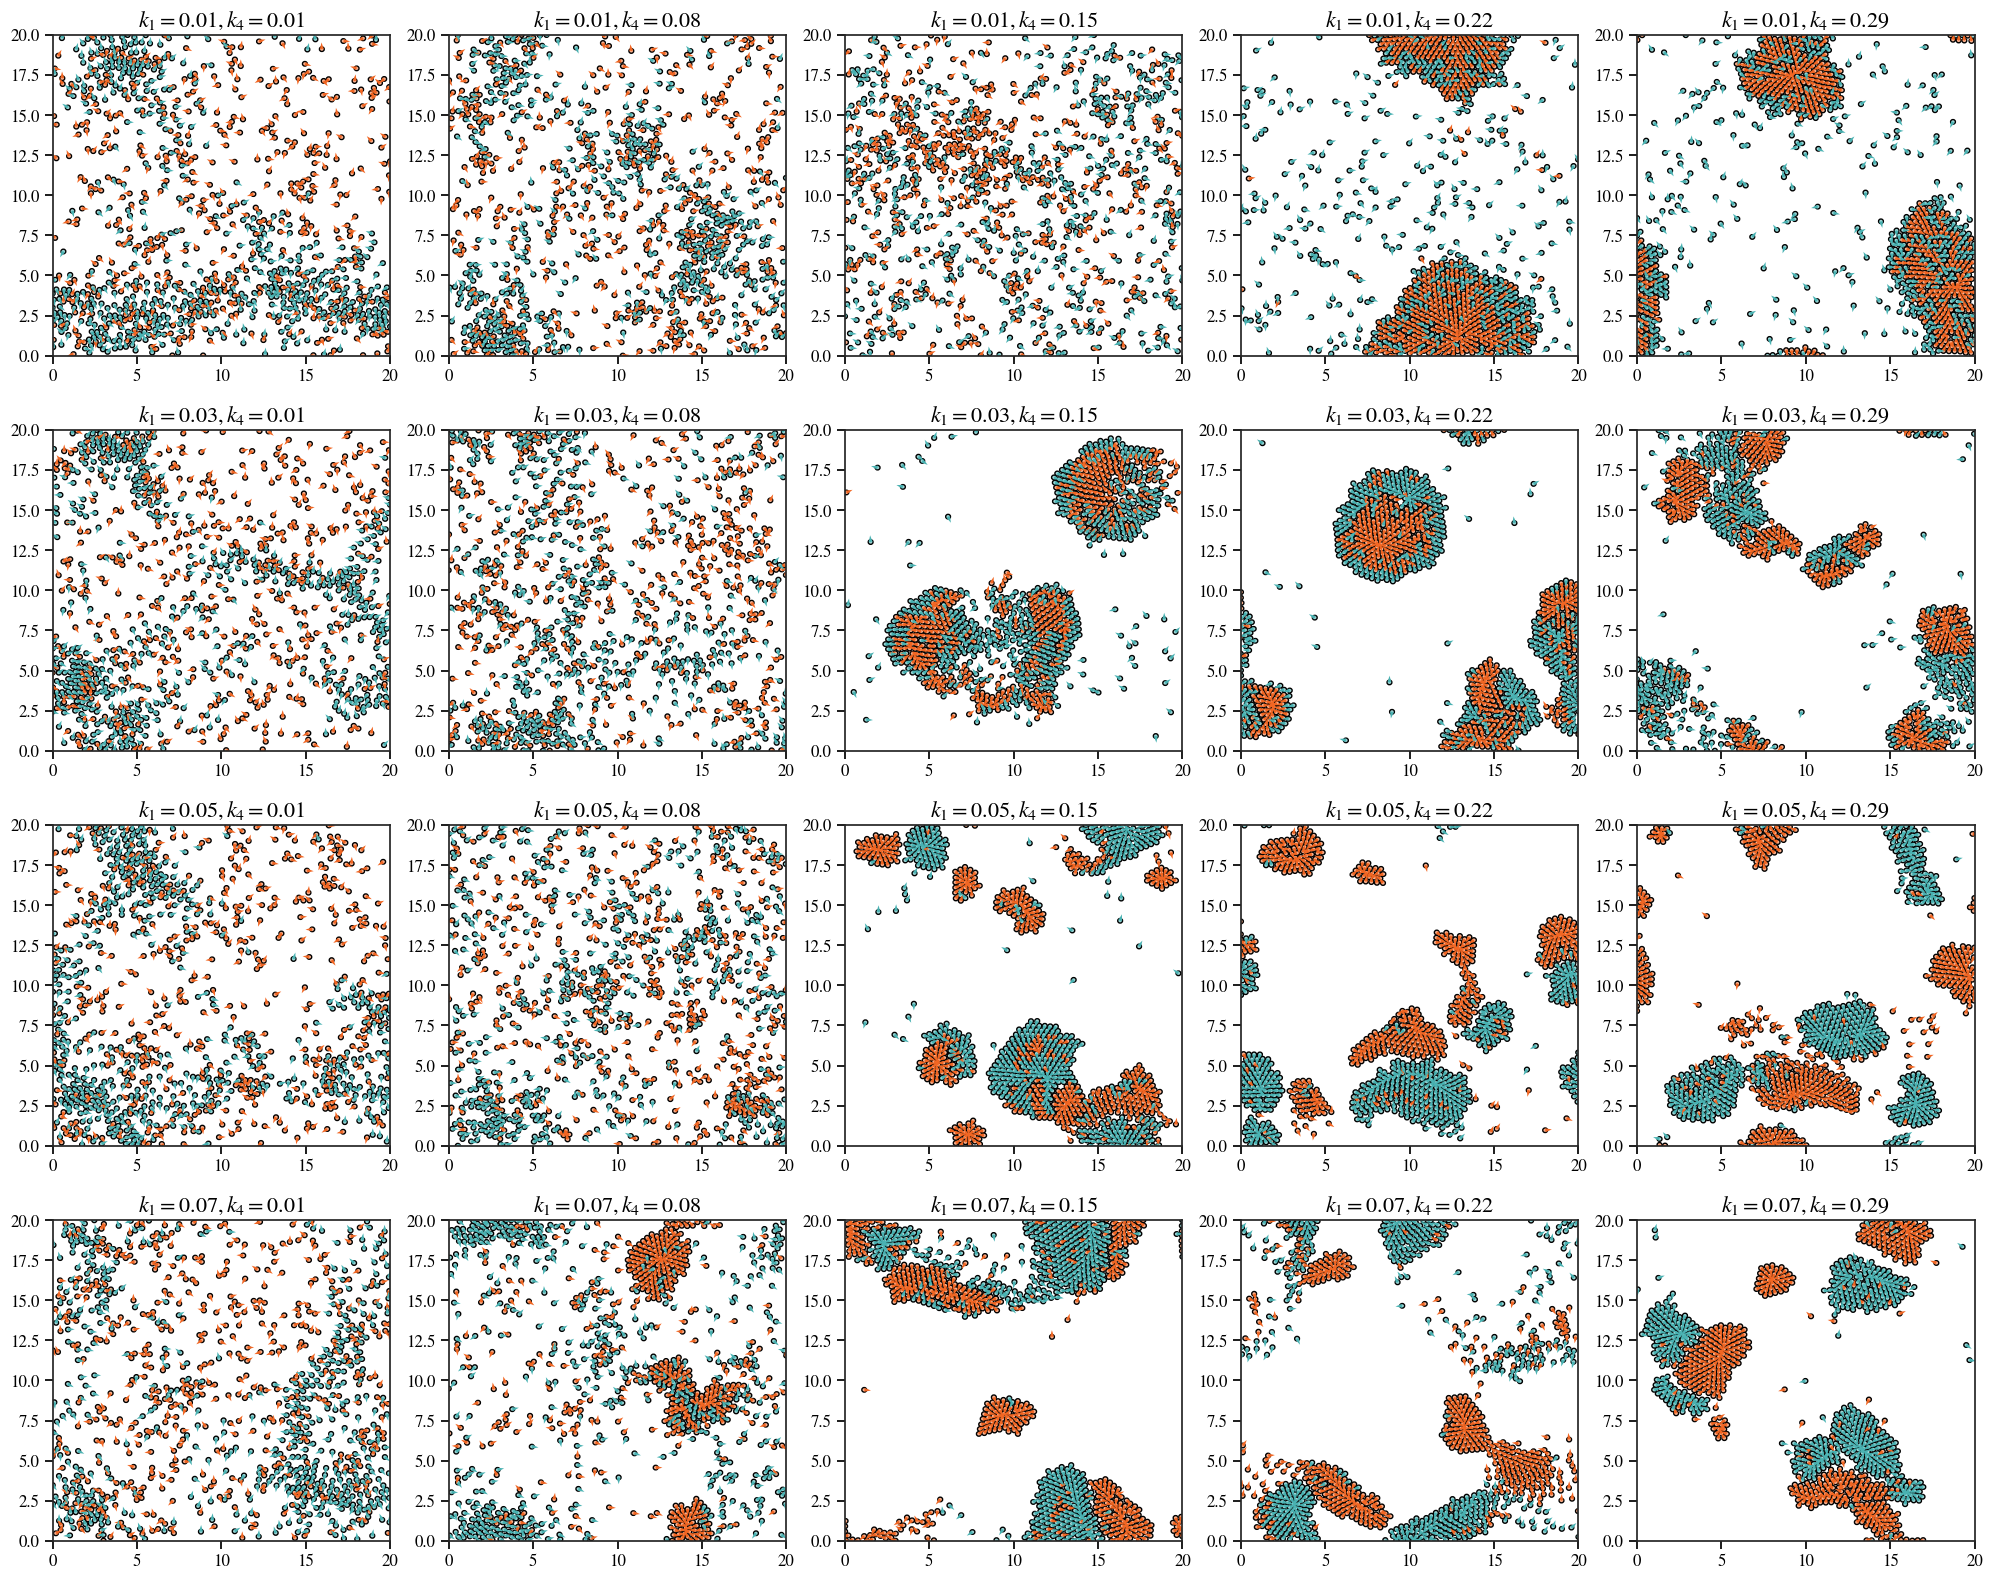
\includegraphics[width=\textwidth]{figs/bigGraphParticle_k23_0.5.png}
\end{figure}

% \bibliography{ref}

\end{document}